\section{Experimental Setup and Measurements}

As explained in Section \ref{sec:theory}, the primary laser 
under examination consists of three essential components. These 
include the laser tube, filled with laser medium, the resonator, 
which is constructed with one partically reflecting and one 
fully reflecting mirror, and the pump source, represented in this 
case electrodes. 

Before using the laser, it requieres adjustment. To accomplish this, 
an alignment laser ($\lambda=\SI{532}{\nano\meter}$) with a power 
of $P_\text{green}=\SI{0.2}{\watt}$ and a target screen are positioned
at the end of the optical bench. The alignment laser should be aligned 
with the optical axis of the main laser so that it intersects with 
the holes in the target screen of the primary laser.  

At the end of the laser tube, Brewster windows are positioned. 
These optical components enable the control of light polarization
by minimizing the reflectance of one polarization at a specific
angle of incidence, known as the Brwester angle. Figure \ref{fig:brewster} 
illustrates how a Brewster window operates.

\begin{figure}
    \centering
    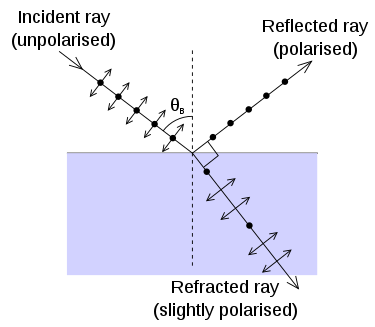
\includegraphics[width=0.5\linewidth]{pictures/Brewster.png} % https://en.wikipedia.org/wiki/Brewster%27s_angle
    \caption{Light path of perpendicularly and parallelly polarized light directed at an interface at the Brewster angle $\theta_\text{B}$.}
    \label{fig:brewster}
\end{figure}

\subsection{Examination of the Stability Condition}
To examine the stability condition, the resonator length is increased
while measuring the laser intensity with a photodiaode. This 
procedure is performed for different mirrors with varying curvature 
radii.

\subsection{Observation of the TEM Modes}
To examine the different modes, a wire (diameter $d=\SI{0.005}{\milli\meter}$)
is positioned between the laser tube and the mirror. After expanding 
the beam with a scattering lense, modes can be identified on the screen. 
Then the screen is replaced with a photodiode to measure the intensity
distribution. This procedure is repeated for two modes.

\subsection{Determination of the Polarisation}
To measure the intensity dependence on the polarization direction, a 
polarizer is positioned between the laser and the photodiode. This 
polarizer is used to set the polarization direction to be measured.

\subsection{Multimode Operation and Frequency Spectrum of the Laser}

A high-speed photodiode (bandwidth up to $\SI{1}{\giga\hertz}$) is 
utilized to measure the beat frequencies for various resonator length. 
The Fourier spectra are subsequently analyzed using a spectrum analyzer.

\subsection{Determining the Wavelength}
To determine the wavelength of the laser, various gratings and slits are 
positioned in the beam. The distance between the diffraction maxima is 
subsequently measured.